\chapter{Conclusions}
In this project, we have achieved touchless interaction between the drone and our hands. We implemented a machine learning model, specifically MediaPipe, for hand tracking. Our gesture recognition model underwent training and testing, and the confusion matrix presents its accuracy. The process is composed of 5 steps: 
\begin{enumerate}[label=\Roman*.]
    \item Drone capturing an image
    \item Image processing via OpenCV
    \item Gesture recognition
    \item Gesture - command conversion
    \item Command execution
  
\end{enumerate}
 Gesture recognition is used in various sectors, including smart home automation and the medical field. It mainly focuses on human-machine interaction. The system receives input images from a drone camera connected to the device. The main goal of this project is to propose a real-time system with high accuracy. 
In summary, the project demonstrates how we can control a drone in an entertaining and educational way. 
\begin{figure}
	\centering
	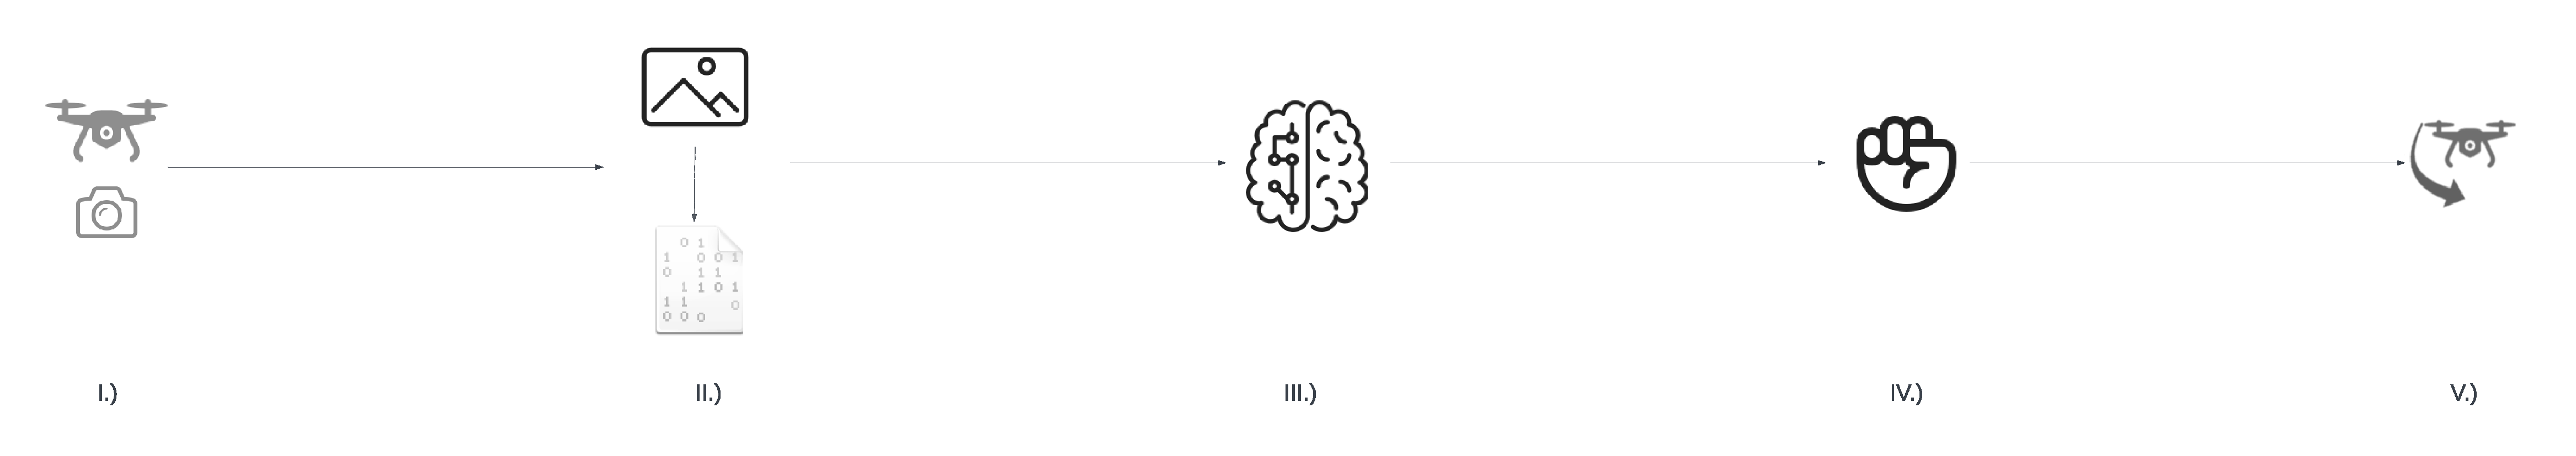
\includegraphics[width = \textwidth]{images/steps.pdf}
	\caption{Steps of the process}
	\label{fig:conclusion}
\end{figure}
\clearpage